\documentclass[../AISTR.tex]{subfiles}

\begin{document}
\section{Реализация обмена сообщениями в среде QT}
\subsection{Сигналы и слоты}
\textbf{Сигналы и слоты} используются для коммуникации между объектами в Qt: 
\begin{itemize}
	\item \textbf{сигнал}: вырабатывается когда происходит определенное событие;
	\item \textbf{слот}: функция, которая вызывается в ответ на определенный сигнал.
\end{itemize}
На \refris{fig:signal-slot} показан механизм работы сигналов и слотов. 
\begin{figure}[h]
	\centering
	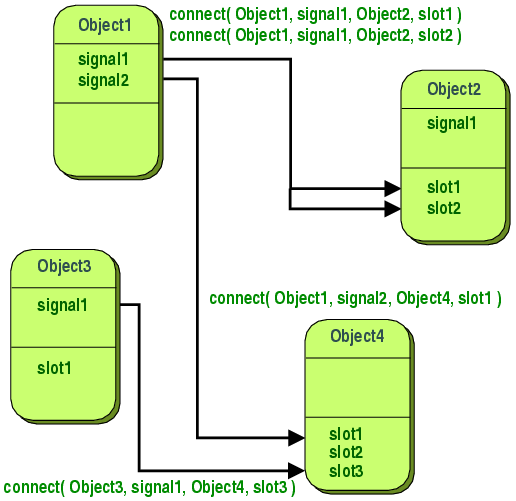
\includegraphics[width=0.7\linewidth]{../images/signal-slot}
	\caption{Схема действия сигналов и слотов}
	\label{fig:signal-slot}
\end{figure}
Здесь
\begin{itemize}
	\item \textit{Object\textsubscript{1}, Object\textsubscript{2}} -- объекты, имеющие в себе сигналы и слоты; 
	\item \textit{connect (args)} -- функция, соединяющая сигналы и слоты в первом и втором объекте
\end{itemize}

\subsection{Концепция программы}
\textbf{Концепция программы} -- реализовать пересылку сообщений между двумя объектами одного класса. 

Первый объект будет отправлять второму сигнал \textit{ping}, а второй первому -- сигнал \textit{pong}.
\subsection{Реализация кода на языке Qt}
\subsubsection{Структура класса}
В листинге \rbf{list:sig_slot} приведён отрывок программы \pp. 
\begin{lstlisting}[caption=Сигналы и слоты класса,captionpos=b, label={list:sig_slot}]
public  slots:
	void processPing(const QString& msg);
	void processPong(const QString& msg);
	void sendPing();
	
signals:
	void ping(QString = "", int = 0);
	void pong(QString);
	void msgPinged(QString);
	void msgPonged(QString);
\end{lstlisting}	
Здесь содержатся 4 сигнала и 3 слота:
\begin{itemize}
	\item \textbf{Сигналы:}
	\begin{enumerate}
		\item \textit{ping} -- сигнал, отправляемый слотом \textit{sendPing};
		\item \textit{pong} -- сигнал, отправляемый слотом \textit{processPing} (см. листинг \rbf{list:slot_processPing});
		\item \textit{msgPinged} -- сигнал графического интерфейса, отправляемый слотом \textit{sendPing} (см. листинг \rbf{list:slot_sendPing});
		\item \textit{msgPonged} -- сигнал графического интерфейса, отправляемый слотом \textit{processPong} (см. листинг \rbf{list:slot_processPong}).
	\end{enumerate}
	\item \textbf{Слоты:}
	\begin{enumerate}
		\item \textit{processPing} -- получает сигнал \textit{ping} и отсылает сигнал \textit{pong}:
		
		\begin{lstlisting}[caption=Реализация слота processPing,captionpos=b, label={list:slot_processPing}]
		void MainClass::processPing(const QString& msg)
		{
			emit pong(msg);
		}				
		\end{lstlisting}	
		\item \textit{processPong} -- получает сигнал \textit{pong} и приступает к его обработке: записывает в строку номер сообщения и время его получения:
		\begin{lstlisting}[caption=Реализация слота processPong,captionpos=b, label={list:slot_processPong}]
		void MainClass::processPong(const QString& msg)
		{
			// ? Display pong process
			QString m;
			m.append("Message ponged # ");
			m.append(QString::number(a));
			m.append(". Time: ");
			m.append(QTime::currentTime().toString("hh:mm:ss"));
			emit msgPonged(m);
			
		}			
		\end{lstlisting}
		\item \textit{sendPing} -- слот, соединённый с таймером, отправляет сигналы \textit{pong} и \textit{msgPinged}:
		\begin{lstlisting}[caption=Реализация слота sendPing,captionpos=b, label={list:slot_sendPing}]
		void MainClass::sendPing()
		{
			++a;
			emit ping(QString::number(a));
			QString m;
			m.append("Message pinged # ");
			m.append(QString::number(a));
			m.append(". Time: ");
			m.append(QTime::currentTime().toString("hh:mm:ss"));
			emit msgPinged(m);
		}
		\end{lstlisting}
	\end{enumerate}
\end{itemize}


\subsubsection{Связь сигналов и слотов}
Для работы с сигналами и слотами, они должны быть соединены между собой. Соединение сигналов и слотов класса между собой приведены в листинге \rbf{list:connect}:


\begin{lstlisting}[caption=Соединение сигналов и слотов,captionpos=b, label={list:connect}]
QObject::connect(&timer, SIGNAL(timeout()),
		&test1, SLOT(sendPing()));

QObject::connect(&test1, SIGNAL(ping(QString)),
		&test2, SLOT(processPing(QString)));

QObject::connect(&test2, SIGNAL(pong(QString)),
		&test1, SLOT(processPong(QString)));

QObject::connect(&test1, SIGNAL(msgPinged(QString)),
		ui->plainTextEdit, SLOT(appendPlainText(QString)));

QObject::connect(&test1, SIGNAL(msgPonged(QString)),
		ui->plainTextEdit_2, SLOT(appendPlainText(QString)));		
\end{lstlisting}
Принцип работы программы следующий (см. \refris{fig:pp-scheme}):
\begin{enumerate}
	\item Вызывается таймер;
	\item Таймер вызывает слот \textit{sendPing};
	\item Слот \textit{sendPing} отправляет сигнал \textit{ping}, а также отправляет сигнал графическому интерфейсу \textit{msgPinged};
	\item Сигнал \textit{ping} вызывает слот \textit{processPing};
	\item Слот \textit{processPing} отправляет сигнал \textit{pong};
	\item Сигнал \textit{pong} вызывает слот \textit{processPong};
	\item Слот \textit{processPong} отправляет сигнал графическому интерфейсу \textit{msgPonged}
\end{enumerate}


\begin{figure}[p]
	\centering
	\includegraphics[trim=80 480 200 60,clip,width=0.5\linewidth]{"../images/схема пингпонг"}
	\caption{Структурная схема программы}
	\label{fig:pp-scheme}
\end{figure}
\subsubsection{Графический интерфейс и окно вывода}
На \refris{fig:pp} показан интерфейс программы до начала работы и после её окончания.

В левом поле пишутся сообщения класса \textit{ping}, в правом -- \textit{pong}. Нижнее поле предназначено для задания интервалов отправки сообщений в милисекундах.

\begin{figure}[p]
	\begin{subfigure}{0.5\linewidth}
		\centering
		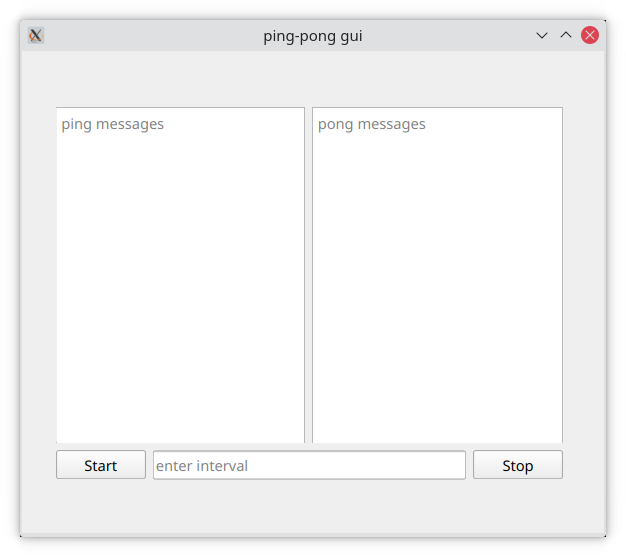
\includegraphics[width=0.9\linewidth]{../images/pp-start}
		\caption{Интерфейс при открытии}
		\label{fig:pp-start}
	\end{subfigure}
	\begin{subfigure}{0.5\linewidth}
		\centering
		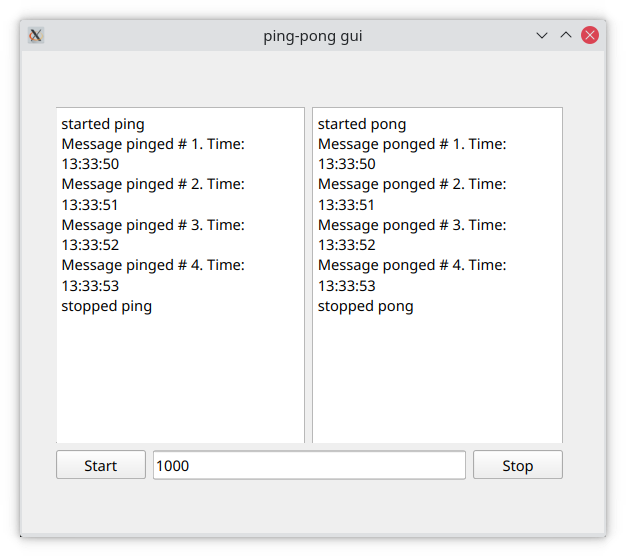
\includegraphics[width=0.9\linewidth]{../images/pp-stop}
		\caption{Интерфейс после исполнения}
		\label{fig:pp-stop}
	\end{subfigure}
	\caption{Графический интерфейс программы}
	\label{fig:pp}
\end{figure}
\end{document}
